\section{Incorporating Sparsity into Scaling Laws}
\label{sec:deriving_scaling_laws}
The scaling laws proposed by \citet{kaplan_scale} provide a framework for predicting loss in dense models by establishing a power-law relationship between loss \(L\), number of parameters \(N\) and dataset size \(D\), where \(N\) and \(D\) interact linearly. Formally, the relationship is given by:
\begin{equation}
L(N, D) = \frac{a}{N^{\alpha}}  + \frac{b}{D^{\beta}} + e
\label{eq:loss:dense}
\end{equation}
Here, the term \(N^{\alpha}\) captures the inverse relationship between model size and loss, where an increase in model size \(N\) leads to a reduction in loss. The exponent \(\alpha\) quantifies the rate of this decrease; a larger \(\alpha\) suggests a steeper reduction in loss with increasing model size. Similarly, the term \(D^{\beta}\) indicates the impact of dataset size \(D\) on loss, with larger datasets contributing to lower loss values. The exponent \(\beta\) measures this relationship, where a larger \(\beta\) implies a greater benefit from increased data. The constant \(e\) represents an asymptotic minimum for the loss, as both model size and dataset size approach infinity.


For dense models with a fixed total training \flops, \(C\), the parameters \(N\) and \(D\) are interrelated through the equation for estimating \flops per example, given as \(C = 6ND\) for transformers.
However, in \moes (Mixture of Experts models), this relationship involves the active number of parameters \(N_a\) rather than the total parameter count \(N\). Thus, \(D\) and \(N_a\) define the total training \flops rather than \(D\) and \(N\).
Given the analysis conducted in \S\ref{sec:n_s_d_interaction}, we know that if the total number of parameters $N$ is fixed, the optimal sparsity level, i.e., active number of parameters would depend on $N$. Motivated by this observation, we suggest the following parametric form  that includes a multiplicative interaction between $N$ and $S$ or $N_a$ to predict the loss:

\begin{equation}
    L(N, D, S) = \frac{a}{N^{\alpha}}  % c, \lambda in NB
                + \frac{b}{D^{\beta}}
                + \frac{c}{\left(1-S\right)^{\lambda}}  % a, \alpha in NB
                + \frac{d}{\left(1-S\right)^{\delta}N^{\gamma}}
                + e
    \label{eq:loss:moe:proposal1}
\end{equation}
The term $\left(1-S\right)$ in the above equation provides a rough estimate of the percentage of active parameters. If the exponent for the multiplicative terms is the same then that term provides an approximate estimate of the number of active parameters.

By incorporating sparsity into the scaling law equation, we can eliminate the need for parameters specific to \moes, such as the total and active number of experts. As demonstrated by \citet{frantar2024scaling}, this formulation also holds for other sparsity mechanisms, such as weight sparsity, where individual neural network connections are pruned.

We use the recipe described by~\citet{hoffmann2022training} and use the L-BFGS algorithm to fit the coefficients in~\eqref{eq:loss:moe:proposal1} using a Huber loss with $\delta=10^{-3}$. Optimal coefficient values were determined through a grid search (see \Cref{tab:lbfgs:hparams} for search values). The results of data fitting and validation are shown in~\Cref{fig:scaling_law}. The estimated values are shown in~\Cref{tab:lbfgs:estimate_params} in~\Cref{appendix:scaling_law_sparsity}. 

\begin{figure*}[ht]
    \centering
    \subfigure[Fit on data used to estimate coefficients.]{
        \label{fig:scaling_law:interpolation}
        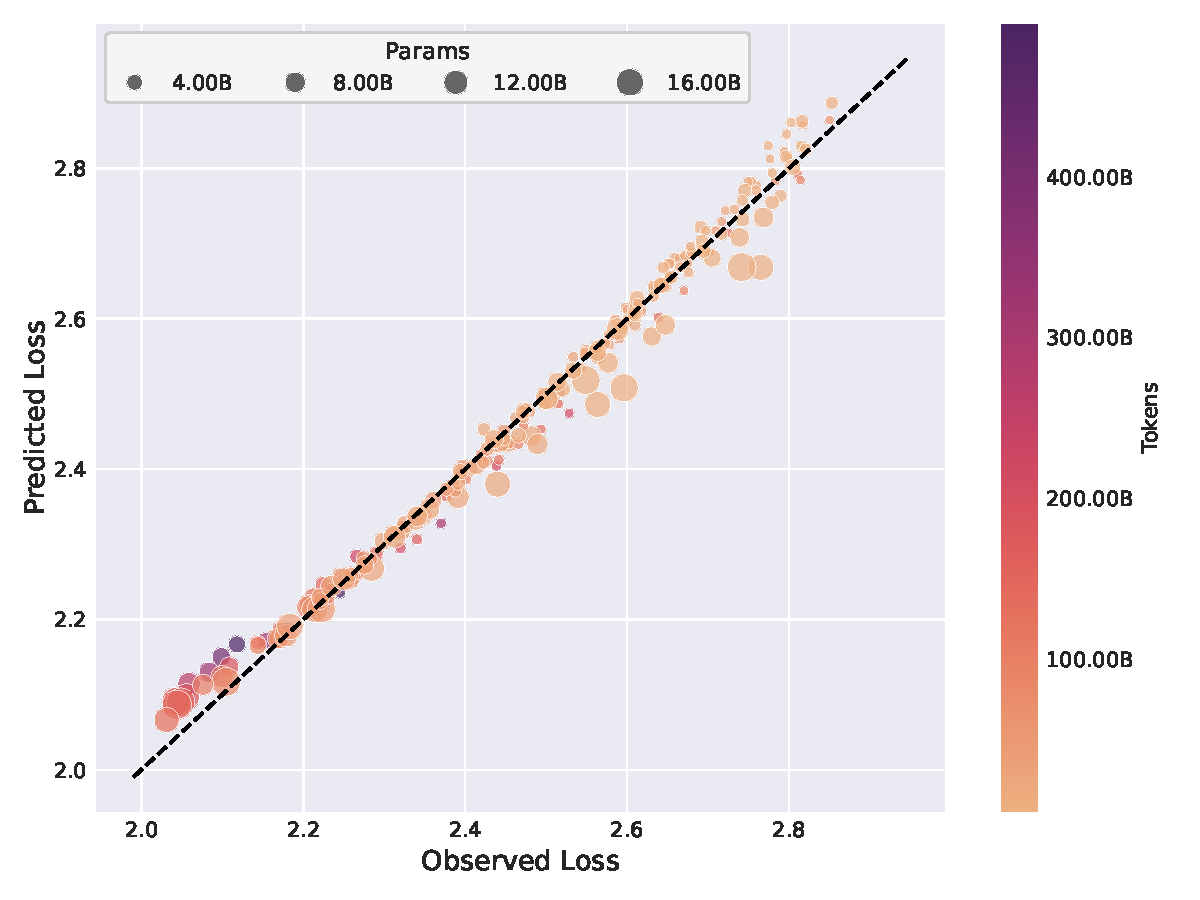
\includegraphics[width=0.45\textwidth]{plots/parameteric_law_interpolation.pdf}
    }
    \quad %\hfill
    \subfigure[Validating scaling law on held-out dataset.]{
        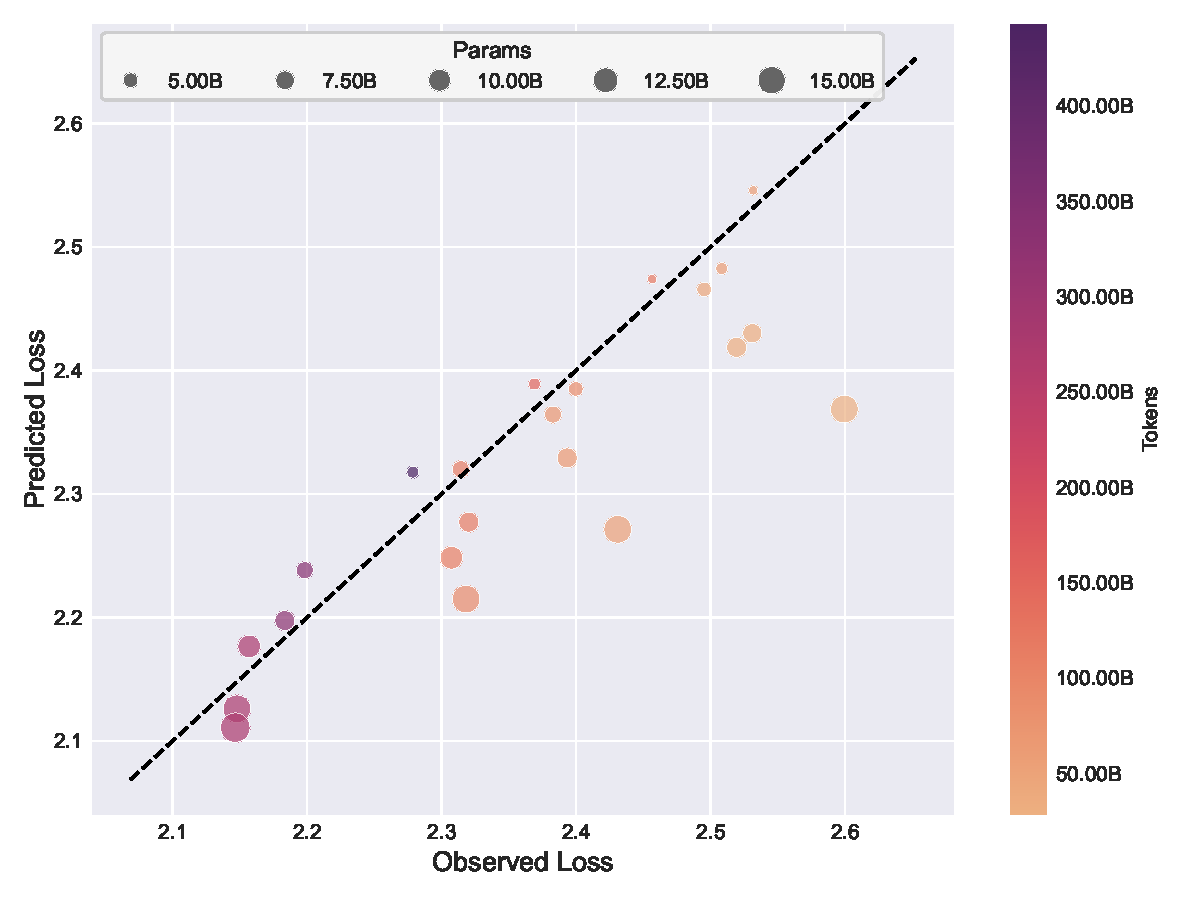
\includegraphics[width=0.45\textwidth]{plots/parameteric_law_extrapolation.pdf}
        \label{fig:scaling_law:sparsity98}
    }
    \caption{Scaling law fit on data obtained from training compute-optimal models. \Cref{fig:scaling_law:interpolation} shows the fit on the data used to estimate the coefficients for \eqref{eq:loss:moe:proposal1}, while \Cref{fig:scaling_law:sparsity98} validates these coefficients on a held-out dataset. All data points with \(S = 0.98 \) were excluded from the fitting process for out-of-sample validation.  The dashed lines represent equal loss values.}
    \label{fig:scaling_law}
\end{figure*}

